\documentclass[oneside,a4paper]{book}

\usepackage{float}


%=============================================================================


\usepackage{amsthm}
\usepackage{xspace}
\usepackage{float}
\usepackage{ifthen}
\usepackage{amsbsy}
\usepackage{amssymb}
\usepackage{balance}
\usepackage{booktabs}
\usepackage{graphicx}
\usepackage{rotating}
\usepackage{multirow}
\usepackage{needspace}
\usepackage{microtype}
\usepackage{bold-extra}
\usepackage{geometry}
\usepackage{varioref}
\usepackage[table,xcdraw]{xcolor}
\usepackage{textcomp}
\usepackage{listings}
\usepackage[normalem]{ulem} %emphasize still italic
\usepackage{ucs}

% \usepackage[utf8]{inputenc}
% \usepackage[htt]{hyphenat}
\usepackage{times}
\usepackage{url}
\usepackage{alltt}
\usepackage{amsmath}
\usepackage{xfrac}
\usepackage{appendix}
\usepackage{stmaryrd}   % for the \shortuparrow
\usepackage[utopia]{quotchap}

\usepackage{setspace}
\usepackage[numbers, sort&compress]{natbib}

\usepackage{mdwlist}        % support for better spaced lists
% allows for temporary adjustment of side margins
\usepackage{chngpage}
\usepackage[normalem]{ulem} 

% algorithmicx ( https://tex.stackexchange.com/questions/163768/write-pseudo-code-in-latex )
\usepackage{amsmath}
\usepackage{algorithm}
\usepackage[noend]{algpseudocode}


\usepackage{subcaption}


% constants

\newcounter{qcounter}

% commands
\newcommand{\n}{$\cdot$}
\newcommand{\y}{\checkmark}
\newcommand{\subscript}[1]{$_{\textrm{\footnotesize{#1}}}$}
\newcommand{\superscript}[1]{$^{\textrm{\footnotesize{#1}}}$}
\newcommand{\vertical}[1]{\raisebox{-4em}{\begin{sideways}{#1}\end{sideways}}}

\newboolean{showedits}
\setboolean{showedits}{true} % toggle to show or hide edits
\ifthenelse{\boolean{showedits}}
{
       \newcommand{\ugh}[1]{\textcolor{red}{\uwave{#1}}} % please rephrase
       \newcommand{\ins}[1]{\textcolor{blue}{\uline{#1}}} % please insert
       \newcommand{\del}[1]{\textcolor{red}{\sout{#1}}} % please delete
       \newcommand{\chg}[2]{\textcolor{red}{\sout{#1}}{\ra}\textcolor{blue}{\uline{#2}}} % please change
}{
       \newcommand{\ugh}[1]{#1} % please rephrase
       \newcommand{\ins}[1]{#1} % please insert
       \newcommand{\del}[1]{} % please delete
       \newcommand{\chg}[2]{#2}
}


% ============================================================================
% Put edit comments in a really ugly standout display

\usepackage{xcolor}
\usepackage[normalem]{ulem}
\newcommand{\ra}{$\rightarrow$}


% comments \nb{label}{color}{text}
\newboolean{showcomments}
\setboolean{showcomments}{true}
\ifthenelse{\boolean{showcomments}}
    {\newcommand{\nb}[3]{
        {\colorbox{#2}{\bfseries\sffamily\scriptsize\textcolor{white}{#1}}}
        {\textcolor{#2}{\sf\small$\blacktriangleright$\textit{#3}$\blacktriangleleft$}}}
     \newcommand{\version}{\emph{\scriptsize$-$Id$-$}}
%	 \newcommand{\ugh}[1]{\textcolor{red}{\uwave{#1}}} % please rephrase
%	 \newcommand{\ins}[1]{\textcolor{blue}{\uline{#1}}} % please insert
%	 \newcommand{\del}[1]{\textcolor{red}{\sout{#1}}} % please delete
%	 \newcommand{\chg}[2]{\textcolor{red}{\sout{#1}}{\ra}\textcolor{blue}{\uline{#2}}} % please change
	 \newcommand{\chk}[1]{\textcolor{ForestGreen}{#1}} % changed, please check
	}
    {\newcommand{\nb}[3]{}
     \newcommand{\version}{}
	\newcommand{\chk}[1]{} % changed, please check
	}

% ============================================================================
% Make quotes be italic
\renewenvironment{quote}
    {\list{}{\rightmargin\leftmargin}%
     \item\relax\begin{it}}
    {\end{it}\endlist}

\newcommand{\ttimes}{\ensuremath{\times}}

%=============================================================================

\newcommand{\needlines}[1]{\Needspace{#1\baselineskip}}

% source code
\usepackage{xcolor}
\usepackage{textcomp}
\usepackage{listings}
\definecolor{source}{gray}{0.9}
\lstset{
	language={},
	% characters
	tabsize=3,
	upquote=true,
	escapechar={!},
	keepspaces=true,
	breaklines=false,
	alsoletter={:},
	breakautoindent=true,
	columns=fullflexible,
	showstringspaces=false,
	basicstyle=\footnotesize\ttfamily,
	% background
	frame=single,
    framerule=0pt,
	backgroundcolor=\color{source},
	% numbering
	numbersep=5pt,
	numberstyle=\tiny,
	numberfirstline=true,
	% captioning
	captionpos=b,
	numberbychapter=false,
	% formatting (html)
	moredelim=[is][\textbf]{<b>}{</b>},
	moredelim=[is][\textit]{<i>}{</i>},
	moredelim=[is][\uline]{<u>}{</u>}}
\newcommand{\ct}{\lstinline[backgroundcolor=\color{white},basicstyle=\footnotesize\ttfamily]}
\newcommand{\lct}[1]{{\small\tt #1}}


%----------------------------------------------------------------------------
% references
\newcommand{\tabref}[1]{\hyperref[{tab:#1}]{Table~\ref*{tab:#1}}}
\newcommand{\figref}[1]{\hyperref[{fig:#1}]{Figure~\ref*{fig:#1}}}
\newcommand{\secref}[1]{\hyperref[{sec:#1}]{Section~\ref*{sec:#1}}}
\newcommand{\lstref}[1]{\hyperref[{lst:#1}]{Listing~\ref*{lst:#1}}}
\newcommand{\charef}[1]{\hyperref[{cha:#1}]{Chapter~\ref*{cha:#1}}}
%----------------------------------------------------------------------------

% abbreviations
\tracingcolors 4
\setcounter{tocdepth}{3}
\setcounter{secnumdepth}{3}
\newcommand{\ie}{\emph{i.e.,}\xspace}
\newcommand{\eg}{\emph{e.g.,}\xspace}
\newcommand{\etc}{\emph{etc.}\xspace}
\newcommand{\etal}{\emph{et al.}\xspace}


%\newcommand{\newevenside}{
%	\ifthenelse{\isodd{\thepage}}{\newpage}{
%	\newpage
%        \phantom{placeholder} % doesn't appear on page
%	\thispagestyle{empty} % if want no header/footer
%	\newpage
%	}
%}

\def\stretchfactor{1}
\newcommand{\mychapter}[1]{\setstretch{1}
    \chapter{#1}\setstretch{\stretchfactor}}

%----------------------------------------------------------------------------
\newcommand{\lessSpace}{\vspace{-1em}}
\DeclareGraphicsExtensions{.pdf,.png}
\graphicspath{{images/}}
%\newcommand{\fig}[4]{
%	\begin{figure}[#1]
%		\centering
%		\includegraphics[width=#2\textwidth]{#3}
%		\lessSpace
%		\caption{\label{fig:#3}#4}
%	\end{figure}}

% ===========================================================================


\newcommand{\thesistitle}{Sound Source Localization and Distance
Estimation in Open Environment using
Simulation and AI}
\newcommand{\thesisauthor}{Denis Rosset}
\newcommand{\thesisleiter}{Michael Mäder}
\newcommand{\thesisasst}{Beat Wolf}
\newcommand{\thesissubtitle}{ }
\newcommand{\thesisdate}{July 2023}



% ===========================================================================

\usepackage[ colorlinks=true, urlcolor=black, linkcolor=black,
			citecolor=black, bookmarksnumbered=true, bookmarks=true,
			plainpages=false,
			pdftitle={\thesistitle}, pdfauthor={\thesisauthor},
			pdfsubject={\thesissubtitle}, pdfpagelabels]{hyperref}

\newcommand{\hrref}[2]{\hyperref}
% ===========================================================================
% ===========================================================================


% D O C U M E N T
% % % % % % % % % % % % % % % % % % % % % % % % % % % % % % % % % %
\begin{document}

% T I T L E
% % % % % % % % % % % % % % % % % % % % % % % % % % % % % % % % % %
\begin{titlepage}  
  \begin{center}  
  
%  \begin{figure}[t]  
%  \vspace*{-2cm}        % to move header logo at the top 
%  \center{\includegraphics[scale=0.2]{logos/MSc_quer.png}}
%  \vspace{0.4in}     
%  \end{figure}

    \thispagestyle{empty}
    
    {\bfseries\Huge \thesistitle \par
    \Large \vspace{0.1in} \thesissubtitle \par}

    \vspace{0.3in} 
    \LARGE{\textbf{Master Thesis} \\}
    \vspace{0.4in}

    {\Large \thesisauthor}
    
    \vspace{0.3in}
    {\Large University of Applied Sciences and Arts Western Switzerland \par}
    \vfill
    {\Large \thesisdate \par}
  

  \vspace{0.9in}
 
  % === Logos ==============================================     
%  \begin{figure}[htp]
%    \centering
%    \includegraphics[scale=0.30]{logos/UNI_Bern.png}\hfill
%    \includegraphics[scale=0.30]{logos/UNI_Neuenburg.png}\hfill
%    \includegraphics[scale=0.80]{logos/UNI_Fribourg.png}
%  \end{figure}
  % === // Logos ===========================================    


  \end{center}

\end{titlepage}

\chapter*{\centering Abstract}
\begin{quotation}
\noindent 

Sound source localization is a well-known problem in the field of signal processing. It is used in many domains, such as robotics, surveillance, and military applications. This project aims to create a baseline to develop a system to localize a sound source in an open environment. We base our project on a neural network that takes a spectrogram as input and predicts the position of a vehicle. We train the neural network using a dataset of sounds recorded from vehicles on the street. We also use a simulation to augment the dataset. To make the model safe, we test it against adversarial attacks to understand how it behaves if someone attacks it.

\vspace{215pt}

{\centering
Supervisors:
\vspace{7.5pt}

Michael Mäder: Professor in computer science

Beat Wolf: Professor in computer science
\vspace{7.5pt}

Principals:
\vspace{7.5pt}

Marc-Antoine Fénart: Professor in civil engineering

Gabriel Python: Scientific associate at Rosas
\vspace{7.5pt}

Expert:
\vspace{7.5pt}

Dr. Robert van Kommer

}
\end{quotation}
\clearpage
\chapter*{\centering Acknowledgements}

I want to express my gratitude to my supervisors, Michael Mäder and Beat Wolf, for the opportunity to realize this Master's thesis with their supervision and for their excellent advice during this project. I also want to thank Marc-Antoine Fénart for the help with the baseline definition and the lent material. Additionally, I want to thank Gabriel Python and every member of the Rosas team for their help, advice, and encouragement during this project. 
Finally, I would like to thank my family and friends for the support they provided during the realization of this project.

\newpage

% Acronym table

\chapter*{\centering Acronyms}
\begin{acronym}[TDMA]
    \acro{HEIA-FR}{Haute École d'Ingénierie et d'Architecture de Fribourg} 
    \acro{HES-SO}{Haute École Spécialisée de Suisse Occidentale (University of Applied Sciences and Arts Western Switzerland)}
    \acro{AI}{Artificial Intelligence}
    \acro{DNN}{Deep Neural Network}
    \acro{CNN}{Convolutional Neural Network}
    \acro{GPU}{Graphics Processing Unit}
    \acro{CPU}{Central Processing Unit}
    \acro{RAM}{Random Access Memory}
    \acro{MPEG}{Moving Picture Experts Group}
    \acro{FFMPEG}{Fast Forward MPEG}
    \acro{SSH}{Secure Shell Protocol}
    \acro{RTP}{Real-time Transport Protocol}
    \acro{SFTP}{Secure File Transfer Protocol}
    \acro{FFT}{Fast Fourier Transform}
    \acro{PCM}{Pulse-code Modulation}
    \acro{FGSM}{Fast Gradient Sign Method}
    \acro{WAV}{Waveform Audio File Format}
    \acro{MP4}{MPEG-4}
    \acro{USB}{Universal Serial Bus}
    \acro{MSE}{Mean Squared Error}
    \acro{ReLU}{Rectified Linear Unit}
\end{acronym}




\tableofcontents



\chapter{Introduction}
\label{ch:introduction}
Within the framework of the research project "NPR Teleoperation", the engineers of the HEIA-FR have
developed the first concept in Switzerland of a remote-controlled automated vehicle. However,
teleoperation only makes sense if the vehicle is automated. There can be no teleoperation without
automation (economic factors) just as there can be no automation without teleoperation (legal, technical,
and social factors). ROSAS then created the Autovete (Automatisation de véhicules téléopérés) project,
financed by HEIA-FR, to build up vehicle automation expertise.
For a vehicle to be fully autonomous, the detection of other emergency vehicles is mandatory. To solve this
issue, V2V (Vehicle-to-Vehicle) communication can be used but is not yet integrated into emergency vehicles.
So, to be able to detect such a vehicle, two signals need to be processed: the sound of the emergency siren
and the blinking lights of the vehicle. The first use case of this project focuses only on sound source
distance estimation and localization.

To understand if sound source estimation and localization could work for emergency detection, a
simpler use case has been created for this project. It is the detection of excessively noisy vehicles on the
street. The goal is to measure the sound level of the passing vehicles and compare it with the legal limits. If
a vehicle exceeds the limit, the system can record its license plate and report it to the authorities. This way,
the system can help reduce noise pollution and improve road safety.
To implement this use case, the system requires a microphone array, a camera, and a processing unit. The
microphone array captures the sound signals from different directions and sends them to the processing
unit. The processing unit applies a sound source localization algorithm to estimate the direction and distance
of the sound source. The camera captures the image of the vehicle and performs license plate recognition.
Big improvements in sound source localization with the help of machine learning are being made1 and can be
used to reliably localize the origin of a sound using one or more microphone arrays (multiple microphones operating in tandem).

A non-negligible problem is that the number of real-world datasets with moving sources in an open
environment is limited. A solution is to create the datasets in realistic sound propagation simulation.
To validate and use the model, it should also be tested to see how it reacts against adversarial attacks,
understand how it can be used in a real environment and limit the attack vector.
\section{Motivation}
\label{intro:motivation}

\subsection{Objectives}

\paragraph{3.1} Objective n°1 Dataset according to the baseline

The first objective is to construct a dataset that is coherent with the project's baseline. The dataset should contain the target variable, features, and necessary pre-processing steps such as missing data imputation, data normalization, and feature engineering. This dataset will help create and understand the problem.

\paragraph{3.2} Objective n°2 Model for better sound source localization and distance estimation

The project should use a neural network model to detect the origin of a sound using a microphone array. The neural network should be trained using the dataset created in objective 3.1 and should be able to accurately localize the sound source. The trained neural network model should be evaluated in a real environment to see how it performs. It should also be evaluated to see how dependable it is in localizing sound sources and how it can be improved.

\paragraph{3.3} Objective n°3 The model should be tested to see how it reacts to attacks

The trained neural network model needs to be evaluated by testing it on data that has been modified in some way, such as by adding or removing noise, or by modifying the sound source. The model could also be tested against various types of attacks, such as masking, time-warping, and frequency-shifting.

\section{Challenges}
\label{intro:challenges}

\subsection{Challenge n°1: Realistic datasets}

One of the main challenges in this project is to construct realistic datasets that accurately capture the data in a real-world scenario. The lack of open-source datasets that contain moving sound sources in open-loop environments can make this difficult. To overcome this challenge, the project should use realistic simulations of sound propagation to produce suitable datasets.

\subsection{Challenge n°2: Robust models}

Another challenge is to create a neural network model that can accurately detect the origin of a sound using a microphone array. The trained model should be highly accurate and robust enough to resist adversarial attacks. To assess the model's robustness, the model should be tested on data that has been modified in some way, such as by adding or removing noise, or by modifying the sound source. The model should also be able to accurately localize the sound source despite the attack.

\subsection{Challenge n°3: Adequate evaluation metrics}

The last challenge is to create an evaluation metric that adequately reflects the model's performance. The evaluation metric should take into account the accuracy of sound source localization in a real environment as well as its ability to resist adversarial attacks. The metric should also be able to capture how well the model can provide reliable results in a variety of environments.
\section{Structure of the thesis}


\begin{itemize}
    \item \textbf{Chapter \ref{ch:background}: Background}: This chapter provides an overview of the background knowledge necessary to understand the project, such as the theory of machine learning and sound propagation, and a brief introduction of sound source localization.
    \item \textbf{Chapter \ref{ch:methodology}: Methodology}: This chapter explains the methodology used in the project, such as creating a dataset, creating a simulation, building a neural network model, and evaluating it using an appropriate metric.
    \item \textbf{Chapter \ref{ch:setup}: Setup}: This chapter describes the work done on the project, such as the simulations used to create the dataset, the neural network model used, and the evaluation metrics used.
    \item \textbf{Chapter \ref{ch:results}: Results}: This chapter presents the results of the project, such as the performance of the neural network model and the evaluation metrics.
    \item \textbf{Chapter \ref{ch:conclusions}: Conclusion and future work}: This chapter concludes this project with a discussion of the main results and a summary of the key findings.
\end{itemize}
<<
\newpage{\pagestyle{empty} \cleardoublepage}


\chapter{Background and Litterature}
\label{ch:background}

This chapter introduces technical concepts and background used in the conceptualized solution of the thesis. It also explains the analysis of the needs of the thesis and finds relations with the current state of research in sound source localization systems.

\section{Baseline analysis}

During the first weeks of the thesis, we had the opportunity to place an installation of microphones on the HEIA-FR main building roof. We took that opportunity to design the baseline and analyze how to build a system around it.

After analyzing the road in front of the HEIA-FR main building, we decided to use the baseline to detect the position of vehicles driving on the road. The road is moderately busy, and the vehicles drive at a reasonable speed. The road is also straight, which makes it easier to detect the position of the vehicles. The baseline is shown in Figure \ref{fig:baseline_setup}. This analysis helps provide an intuitive understanding of the sound source localization system. The baseline comprises a vehicle as the sound source we want to record, multiple microphones recording the sound of the street, and an embedded system that manages the microphones.

\section{Sound Source Localization}

Sound Source Localization (SSL) is the process of determining the position of a sound source. It usually uses a microphone array that captures the sound signals from multiple directions. Various applications use SSL \cite{Grumiaux_2022}, such as speech recognition \cite{7952261}, source separation \cite{8903121}, human-robot interaction \cite{Li_2016} or room acoustic analysis \cite{amengual}. In this thesis, SSL is used to estimate the distance and direction of a sound source to detect excessively noisy vehicles.

\subsection{Spectrograms for sound visualization}
\label{subsec:spectrograms}

Spectrograms are a visual representation of the frequency content of a sound signal. They are often used in sound source localization to identify the direction of a sound source. The spectrogram is a two-dimensional representation of the frequency content of a sound signal (figure \ref*{fig:spectrogram_example}).

\begin{figure}[H]
    \centering
    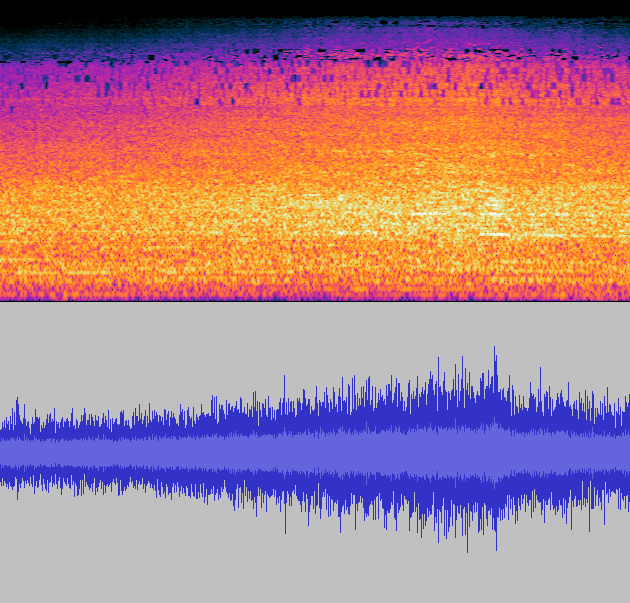
\includegraphics[width=0.5\textwidth]{../Images/spectrogram-example.png}
    \caption{Spectrogram of a sound signal}
    \label{fig:spectrogram_example}
\end{figure}

The x-axis represents time, and the y-axis represents frequency. The intensity of the color at each point in the spectrogram represents the amplitude of the frequency component. A matrix of spectrograms allows the representation of multiple channels, such as the ones recorded by a microphone array. On that matrix, each spectrogram represents the frequency content of a single channel (figure \ref*{fig:2_channel_spectrogram_example}).

\begin{figure}[H]
    \centering
    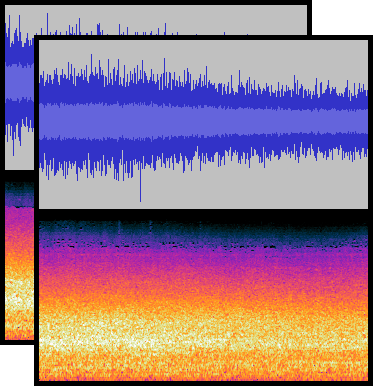
\includegraphics[width=0.4\textwidth]{../Images/2-channel-spectrogram-example.png}
    \caption{Dual channel spectrogram matrix of a sound signal}
    \label{fig:2_channel_spectrogram_example}
\end{figure}

Looking at the frequency content of the sound signal allows us to identify the time delta of a recorded sound by using a multi-channel spectrogram. The bright spot on the spectrogram will indicate a jump in the amplitude and determine the start time of the recording of a loud sound. By comparing this time with the other channel, we can find the direction of the sound source by comparing the sound signal's time delta with the other channels' time delta (figure \ref*{fig:spectrogram_offset}).

\begin{figure}[H]
    \centering
    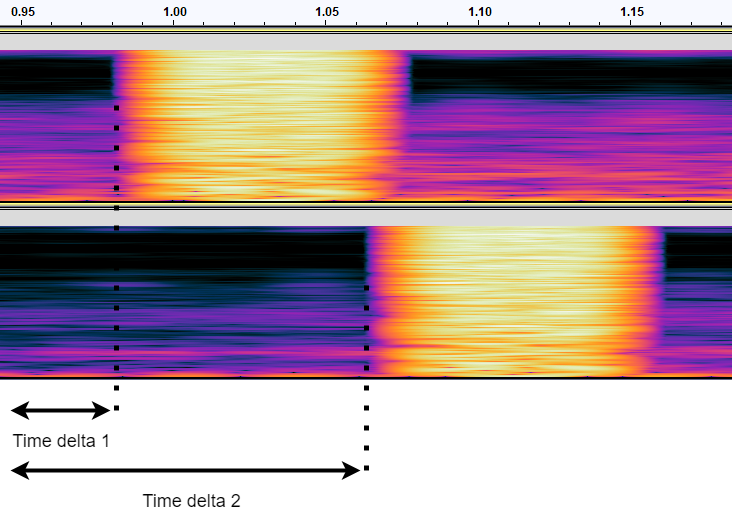
\includegraphics[width=0.5\textwidth]{../Images/time_delta.png}
    \caption{Spectrogram of two sound signals with time their delta}
    \label{fig:spectrogram_offset}
\end{figure}

Since we know the distance between the microphones, we can determine the direction of the sound.

\subsection{Origin of sound using two microphones}

Admitting the following setup (figure \ref*{fig:microphones_setup}), if the time delta 1 is greater than the time delta 2 of the other channels (setup 1), the sound source is closer to microphone 2. If the time delta 1 equals the time delta 2 (setup 3), the sound source is at the same distance to both microphones. If the time delta 2 is greater than the time delta 1 (setup 2), the sound source is closer to the microphone 1. 

\begin{figure}[H]
    \centering
    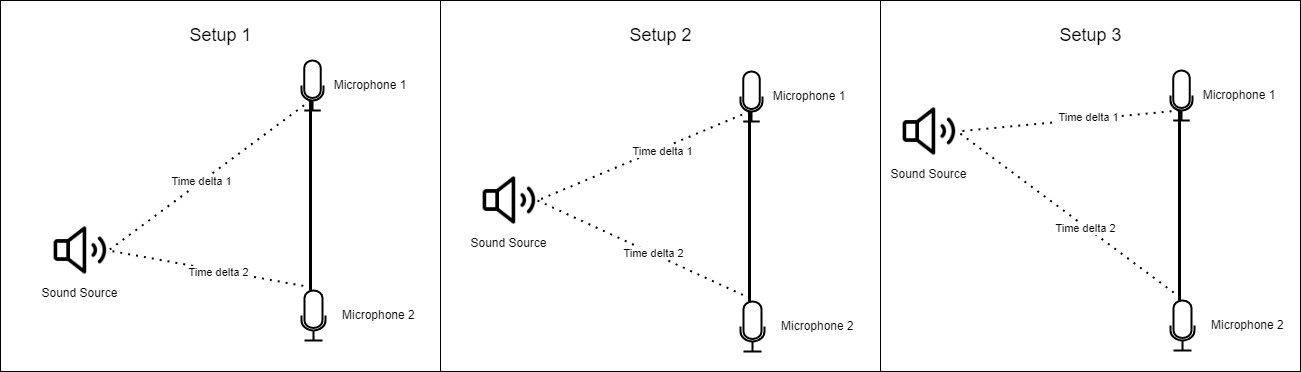
\includegraphics[width=1\textwidth]{../Images/microphones_setups.png}
    \caption{Sound source localization setup}
    \label{fig:microphones_setup}
\end{figure}

This concept can be formalized and is better explained in \cite{Scola2010DirectionOA}. Once the delay between the two microphones is known, the equation allows us to find the direction of the sound source by using trigonometric calculations. As in the figure \ref*{fig:sound-source-from-two-microphones}, considering point $M$ as the sound source and point $A$ and $B$ as microphones, the distance between the two microphones is $d$ and the time delta between the two microphones is $\Delta t$, the angle $\alpha$ can be calculated.

\begin{figure}[H]
    \centering
    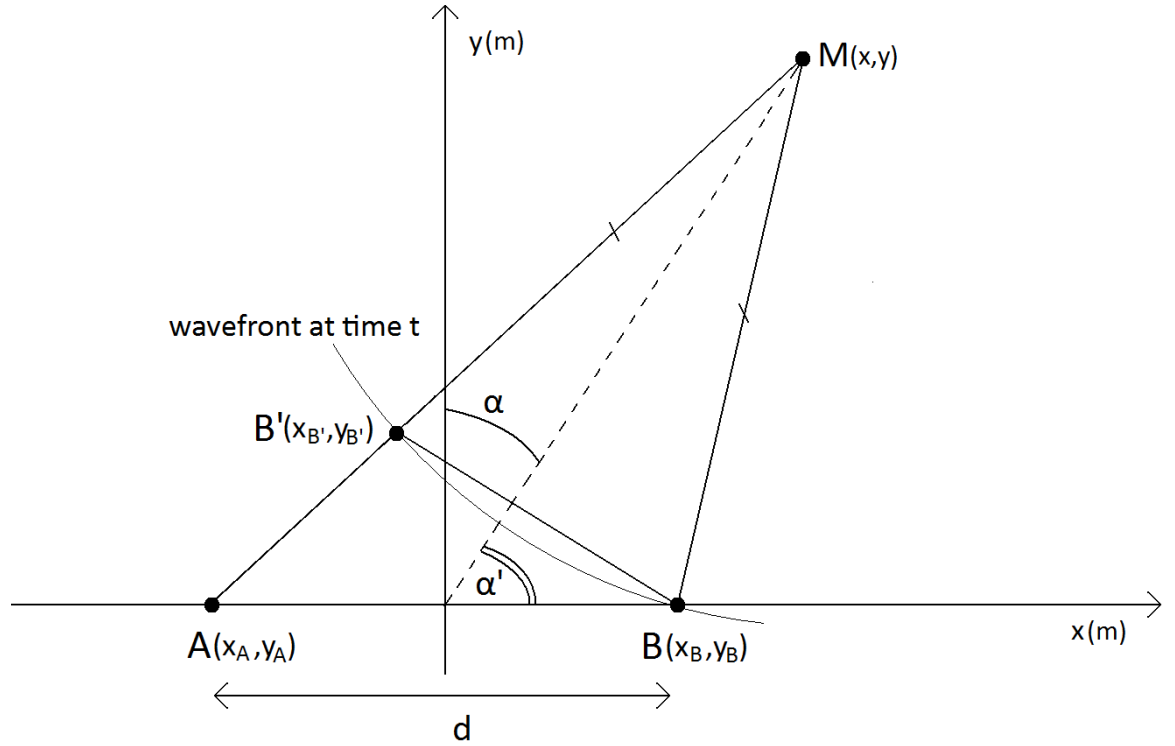
\includegraphics[width=0.7\textwidth]{../Images/sound-source-from-two-microphones.png}
    \caption{Equation formalization. Original image from \cite{Scola2010DirectionOA}}
    \label{fig:sound-source-from-two-microphones}
\end{figure}

Looking at the graphic allows us to find the following equation:

\begin{equation}
    AB' = AM-B'M
\end{equation}

With Pythagorean theorem: 

\begin{equation}
    AM = \sqrt{(X_{a}-X)^2 + (Y_{a}-Y)^2}
\end{equation}
\begin{equation}
    BM = \sqrt{(X_{b}-X)^2 + (Y_{b}-Y)^2}
\end{equation}

The two microphones have the same $Y$ coordinate, so $Y_{a} = Y_{b} = Y$ and $Y_{a}-Y_{b} = 0$ and $X_{a} = -X_{B}$ The equation becomes:

\begin{equation}
    y = \pm\sqrt{\frac{AB'^2}{4} - x^2_{B} + x^2(\frac{4\cdot x^2_{B}}{AB'^2} - 1)}
\end{equation}

This setup shows that two microphones are enough to determine the direction of a sound source.
%!!!!!!! TODO - compléter la formalisation

\section{Neural networks}

The report [A survey of sound source localization with deep learning methods]\cite{Grumiaux_2022} shows that deep neural networks achieve good scores in sound source localization. Neural networks are machine learning algorithms based on biological neurons used to solve various problems, including image recognition, speech recognition, and natural language processing. Neural networks learn from provided data to solve a problem without explicitly programming the solution. Many domains, like self-driving cars, facial recognition, and medical imaging, achieve state of the art results using neural network models. 

A neural network (figure \ref*{fig:neural_network}) is composed of multiple neurons (the circles) that are organized in layers and connected to the neurons in the previous and next layers. 

\begin{figure}[H]
    \centering
    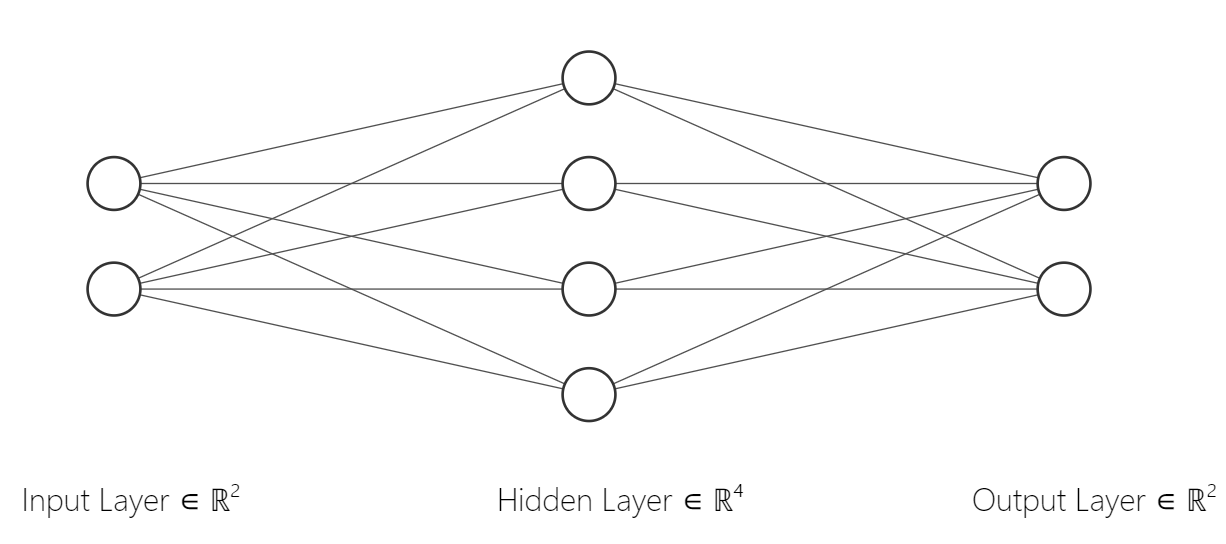
\includegraphics[width=0.7\textwidth]{../Images/neural_network_example.png}
    \caption{Neural network}
    \label{fig:neural_network}
\end{figure}

Neural networks comprise multiple neurons. Neurons are mathematical functions with activation functions and weights. These determine how the neurons respond to inputs and connect to other neurons. Neural networks are trained by adjusting the weights to minimize the error between the predicted and desired outputs, using methods like gradient descent\cite{zhang2019gradient} and backpropagation\cite{Sekhar}.

\subsection{Deep Neural Networks}

Deep neural networks are a type of neural network composed of multiple layers of neurons\cite{Schmidhuber_2015}. They are trained on a large dataset of images and then used to classify new images. There are countless architectures \cite{LIU201711} and implementations of neural networks, but they all share the same basic principles. The most known architectures of neural networks include CNNs\cite{oshea2015introduction}, transformers\cite{vaswani2017attention}, and many others.

\subsection{Convolutional Neural Networks for sound source localization}

Convolutional Neural Networks (CNNs)\cite{oshea2015introduction} are deep neural networks specifically used for image recognition. They are often composed of convolutional, subsampling, and fully connected layers (Figure \ref*{fig:cnn_example}).
\begin{itemize}
    \item{} Convolutional layers are used to extract features from images. These features are then fed into fully connected layers to perform classification. Each convolutional layer comprises multiple filters convolved with the input image to produce a feature map. The filters are trained to extract specific features from the input image.
    \item{} Subsampling layers are used to reduce the size of the feature maps. The most common subsampling layer is the max-pooling layer, which takes the maximum value of a specific region of the feature map.
    \item{} Fully connected layers are trained to classify the features extracted by the convolutional layers. The output of the fully connected layers is a probability distribution over the possible classes. 
\end{itemize}

\begin{figure}[H]
    \centering
    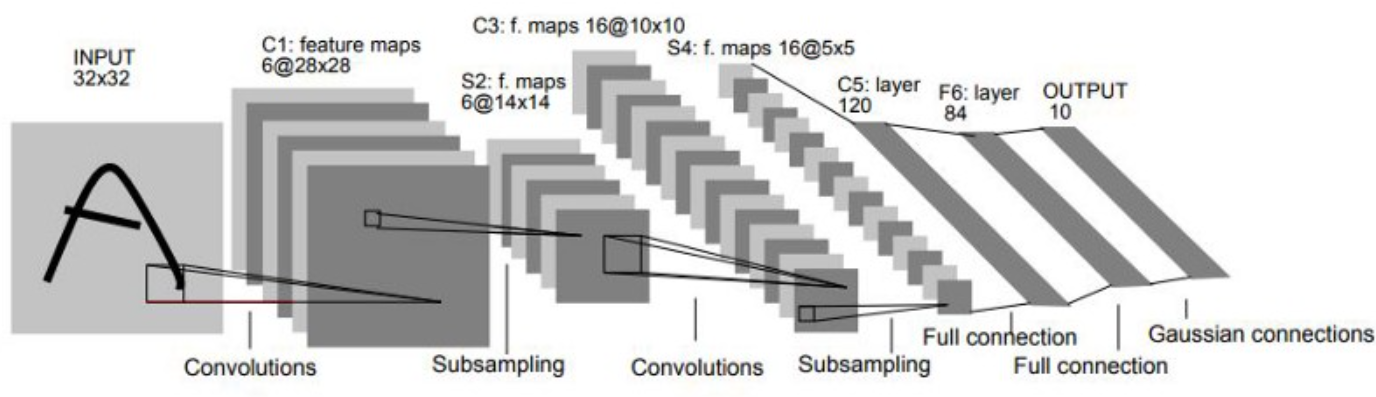
\includegraphics[width=0.7\textwidth]{../Images/cnn_example.png}
    \caption{CNN architecture example with LeNet-5 \protect\cite{726791} composed of two convolutional layers, two subsampling layers, and finishing with two fully connected layers.}
    \label{fig:cnn_example}
\end{figure}

Even if CNNs are mainly used to classify photography, they can classify any images, including sounds\cite{Grumiaux_2022}. Based on section \ref*{subsec:spectrograms}, CNNs can use spectrograms as input since they also are images. The spectrograms are converted into images and fed into the CNN. 

An approach for sound source localization is using classes to define zones where the sound can come from as the classes. The CNN will output a probability distribution over the possible classes. The class with the highest probability is the predicted class. The predicted class can then refer to a zone.

The CNN then outputs a probability distribution over the possible classes. The possible classes need to be defined before training the CNN. In\cite{s20010172}, they approach the problem with 15 classes, using angles 0, 30, and 60 degrees and distances 1, 2, and 3 meters (Figure \ref*{fig:Yiwere_classes}).

\begin{figure}[H]
    \centering
    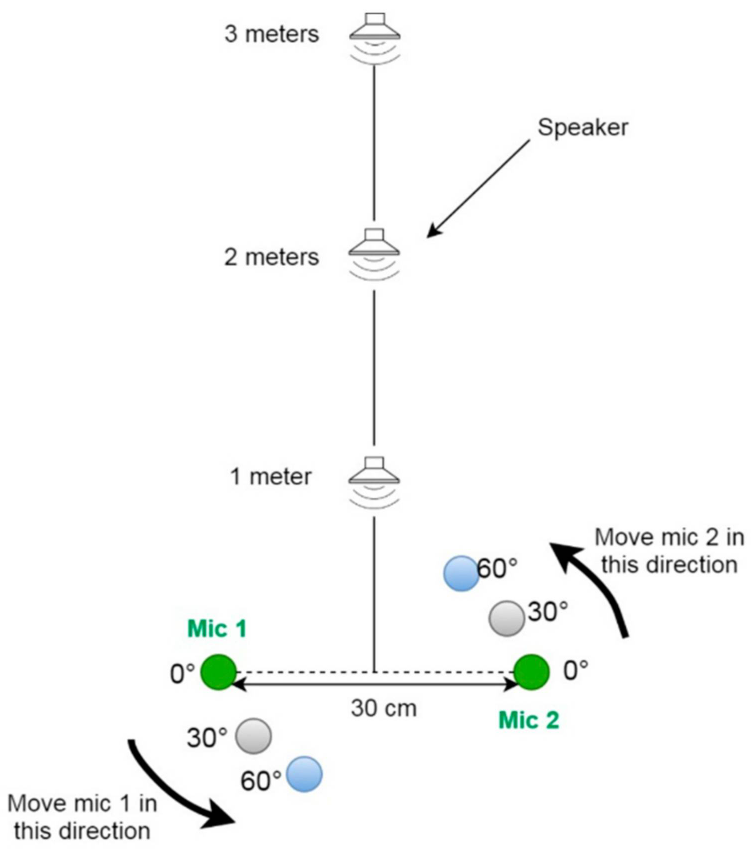
\includegraphics[width=0.7\textwidth]{../Images/Yiwere_classes.png}
    \caption{CNN for source localization}
    \label{fig:Yiwere_classes}
\end{figure}

Based on the baseline defined in chapter \ref*{chap:state_of_the_art}



\subsection{Transfer learning}

%!!!!!!! TODO - réécrire la partie sur le transfer learning
Transfer learning is a machine learning technique where a model trained on a specific task is reused as the starting point for a model on a different task. The model is trained on a large dataset and then used as a starting point for a model on a different dataset. The model is then trained on the new dataset, and the weights are adjusted to minimize the error between the predicted and desired outputs. Transfer learning is used to train models on smaller datasets and achieve better results than training the model from scratch.

\section{Datasets for sound source localization}
\label{sec:datasetsSSL}

Datasets are needed to train and test neural networks. They are composed of data and labels. The data is the neural network input, and the label is the expected output. In the case of sound source localization, the data is audio, and the labels are the zones of the sound source. 

Multiple datasets exist in sound source localization for neural networks. The most common are the DCASE 2019 task 3 dataset\cite{Adavanne2019_DCASE} and the DCASE 2020 task 3 dataset\cite{politis2020dataset}. These datasets are composed of audio files and the corresponding labels. The labels are the zones of the sound source. The audio files are recorded in a room with a microphone array and a sound source. The sound source is moved around the room, and the audio is recorded. The audio files are then annotated with the zones of the sound source. The annotations are done manually by listening to the audio files and annotating the zones. Multiple annotators then verify the annotations to ensure the quality of the annotations. 

Although these datasets are good baselines for sound source localization, they do not suit the needs of this project. The datasets are recorded in a closed environment and do not reflect the baseline defined in this project. Still, these datasets are good baselines for sound source localization and help to understand how to create a dataset.




\subsection{Dataset augmentation for audio classification}
% TODO add sources
Since recording many audio files is time-consuming and costly, and since the dataset needs to be large to train a neural network, we decided to use dataset augmentation techniques.

Dataset augmentation is a technique used to increase the size of a dataset. It is used to improve the performance of a neural network by training on more data, thus becoming better at generalizing. The most common techniques are flipping, rotating, and cropping images, but since the classification in this project is realized on audio, other techniques are needed to augment the dataset. 

Some techniques that work well on audio are adding noise, changing the pitch, or simulating new data. 

\section{Dataset simulation for sound source classification}

Simulating a dataset is a technique used to create a dataset without recording audio from real life. It helps to create a dataset with many samples and labels. Since the goal is to generate sounds in an open environment, a 3D-capable engine is necessary. Game engines are increasingly used for simulation since they are optimized for real-time rendering and can simulate complex 3D scenes. The game engine must simulate sound propagation for a realistic audio simulation.

\subsection{Sound propagation}
Sound propagation is the physical process by which sound waves propagate in a given environment. Multiple factors affect the propagation of sound waves, including reverberation, occlusion, doppler effect, and obstruction.


The strength of the sound wave depends on various factors, including the frequency, environment, and distance from the sound source. These factors make an accurate identification and localization of a sound source difficult; thus, we need a more accurate and robust sound source localization system.

\subsection{Microsoft Project Acoustics}

Microsoft Project Acoustics is a sound propagation engine that simulates the propagation of sound waves in a given environment. Various applications, including video games, virtual reality, and physics simulation, use this engine. It simulates wave effects like obstruction, reverberation, and occlusion in complex 3D scenes without requiring zone markup or raytracing. It works similarly to a raytracing engine but is precomputed and optimized for real-time performance. 

\subsubsection{Sound Propagation in game-engine}

\section{Adversarial Attacks}

Adversarial attacks are a manipulation technique that aims to fool a neural network by modifying the input data. The goal is to make the neural network misclassify. Adversarial attacks allow us to test the robustness of neural networks and understand how neural networks work and how we can improve them.

\subsection{Adversarial attacks categories}

Adversarial attacks can be categorized into white-box attacks and black-box attacks. White-box attacks are attacks where the attacker has access to the neural network's parameters and architecture. Conversely, black-box attacks are attacks where the attacker cannot access the neural network's parameters and architecture.

% Ajouter les sources

\subsection{Fast Gradient Sign Method}

One of the most common adversarial attacks is the Fast Gradient Sign Method (FGSM)\cite{goodfellow2015explaining}. It is a white-box attack that uses the gradient of the loss function to find the adversarial example. The adversarial example is calculated using the following equation:

\begin{equation}
    X_{adv} = X + \epsilon \cdot sign(\nabla_{X}J(\theta, X, y))
\end{equation}

$X$ is the input, $y$ is the target class, $\epsilon$ is the magnitude of the perturbation, and $J(\theta, X, y)$ is the loss function. The loss function is the function that the neural network normally tries to minimize, but here is used to maximize the loss. The gradient of the loss function is calculated for the input $X$. The sign of the gradient is then calculated and multiplied by the magnitude of the perturbation $\epsilon$. The result is added to the input to create the adversarial example $X_{adv}$. The adversarial example is then fed into the neural network, which outputs the adversarial class (Figure \ref*{fig:fgsm}).

\begin{figure}[H]
    \centering
    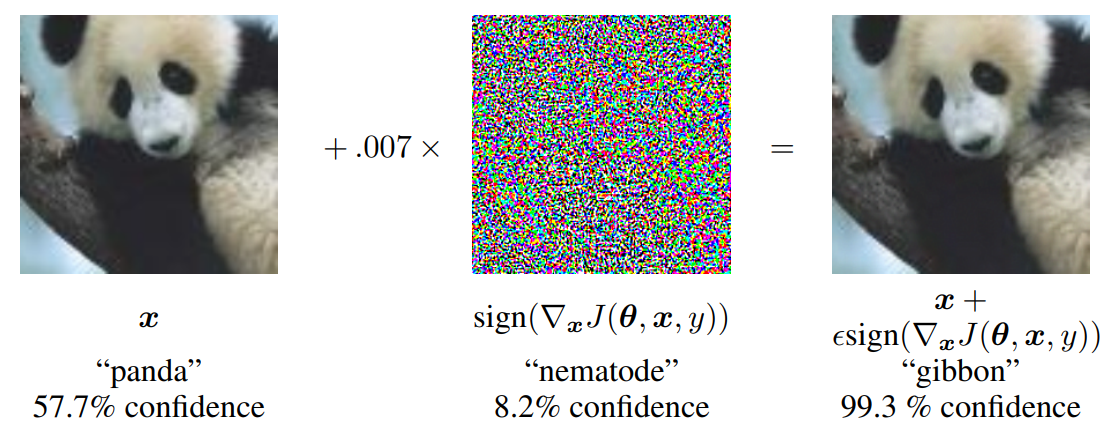
\includegraphics[width=0.7\textwidth]{../Images/fgsm.png}
    \caption{FGSM example in \cite{goodfellow2015explaining} with a neural network classifying a panda as a gibbon because of the attack.}
    \label{fig:fgsm}
\end{figure}

\newpage{\pagestyle{empty} \cleardoublepage}



\chapter{Approach and Design}
\label{ch:methodology}

This chapter presents the design of the project. It is the description of the project's architecture and the project's components.

\section{Baseline design}
\label{sec:baseline_design}

We must design a baseline since we start the project without previous work. The baseline is the starting point of the project. It is the simplest system that we can create to solve the problem. The baseline can then compare the results and improve the system.

\paragraph{Problem statement}

The problem we are trying to solve is to detect and localize a vehicle's sound source in an open environment. 

The baseline system comprises three main parts: the vehicle recordings, the dataset creation, the model training, and the model testing. The system design is shown in Figure \ref{fig:baseline_system_design}.

\begin{figure}[H]
    \centering
    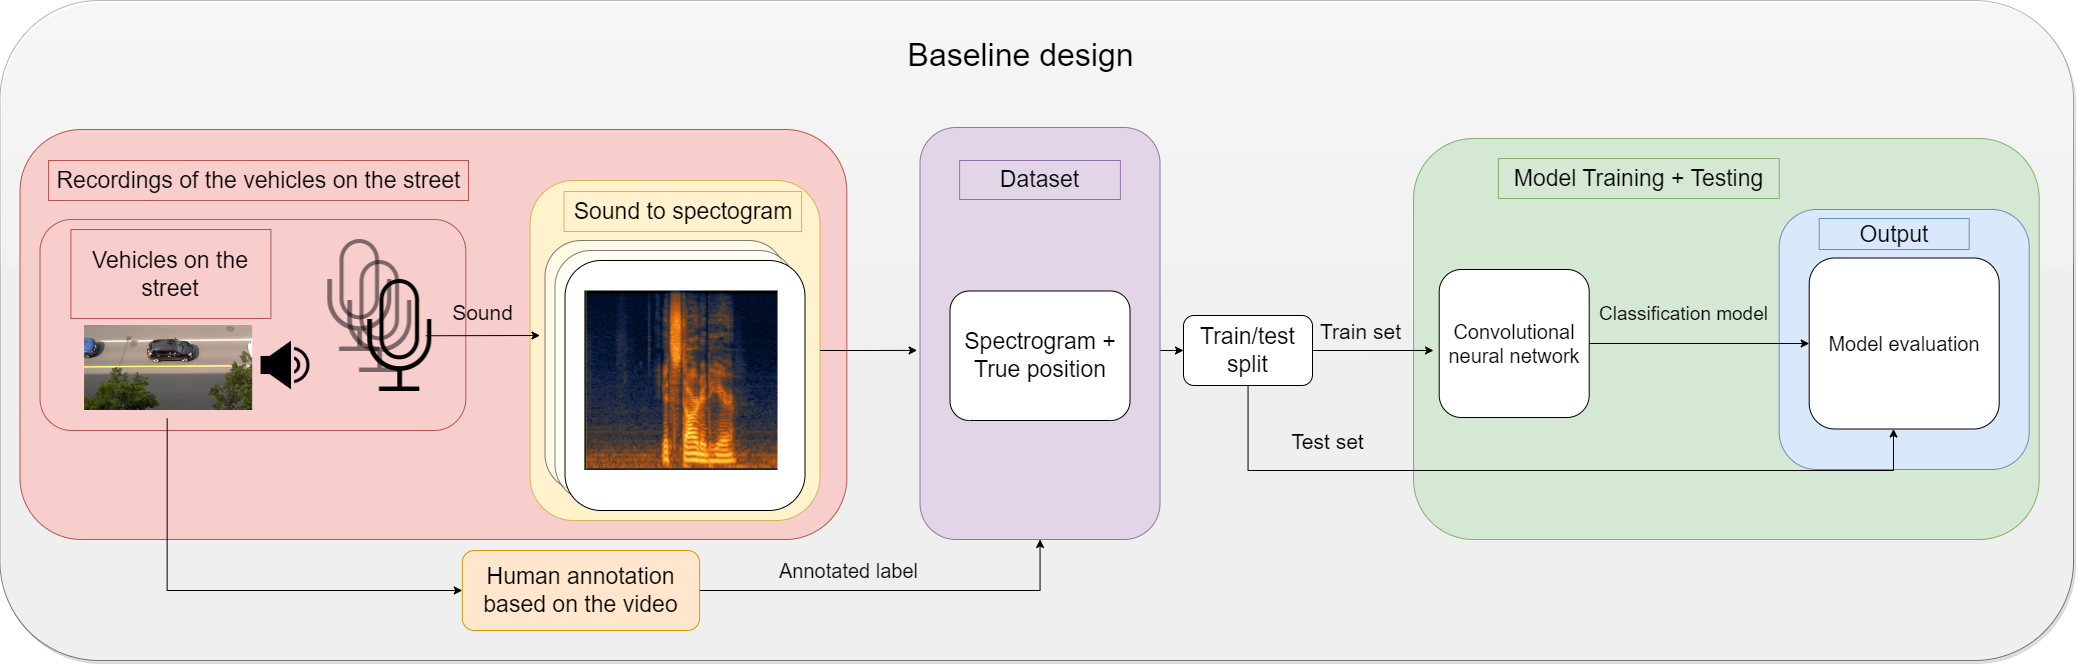
\includegraphics[width=1\textwidth]{../Images/baseline_system_design.drawio.png}
    \caption{Baseline system design}
    \label{fig:baseline_system_design}
\end{figure}

In Figure \ref{fig:baseline_system_design}, the red zone represents the vehicle recordings with multiple microphones and the transformation of the sound into spectrograms. We also record a video to have a ground truth to annotate the dataset. The purple zone represents the dataset creation with the spectrograms as data and the annotations from humans watching the videos as labels. We then split the dataset into a train and a test set. In the green zone, we feed the train set into a neural network to train it to predict the position of the sound source based on the spectrograms. We then test the model on the test set to evaluate its performance with unseen data.

Once we train and evaluate the model, we can use it to predict the position of a sound source based on a new recording. The model can be used in inference to detect the position of a sound source. The inference is shown in Figure \ref{fig:baseline_inference}.

\begin{figure}[H]
    \centering
    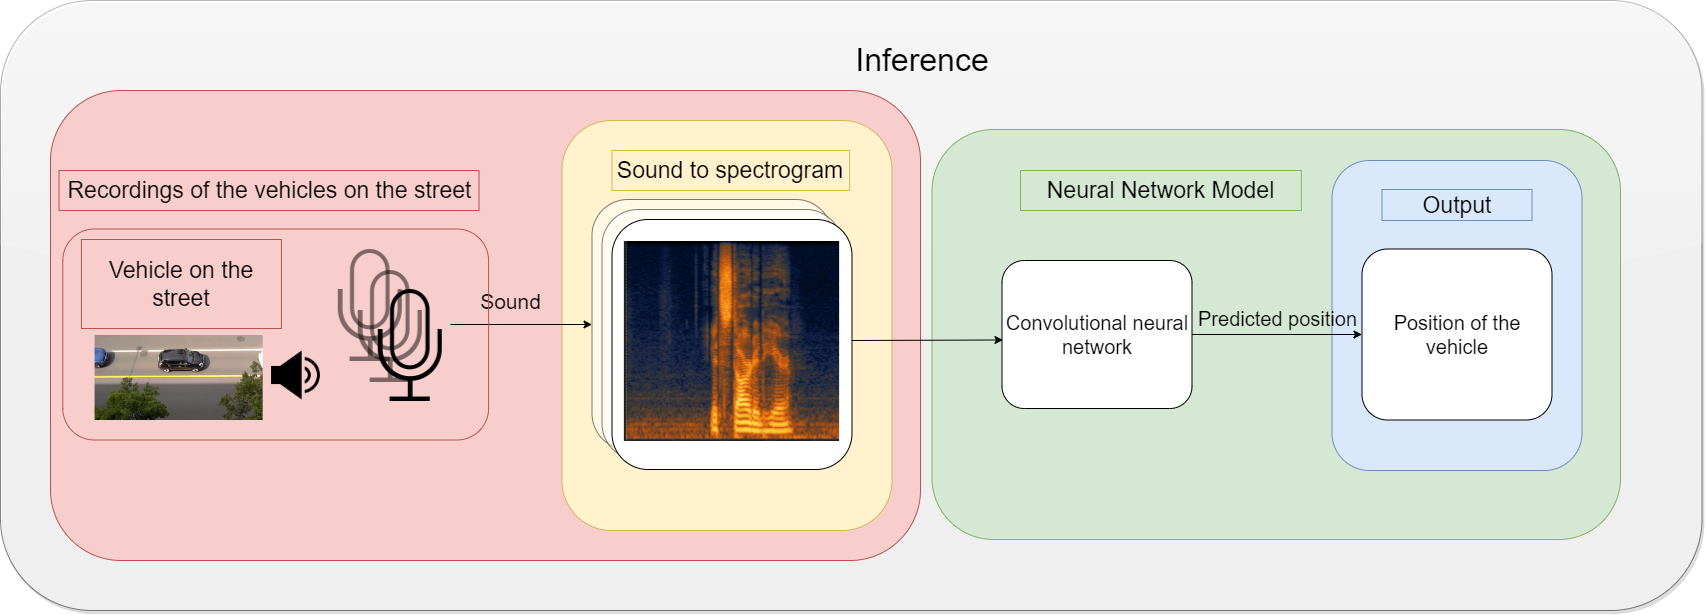
\includegraphics[width=1\textwidth]{../Images/baseline_inference.png}
    \caption{Baseline inference}
    \label{fig:baseline_inference}
\end{figure}

The inference is similar to the training and testing, except that we do not have the ground truth since our model makes the prediction. We only have to do the spectrograms from the recording, and we can feed the spectrograms into the model. The model will then predict the position of the sound source.

We can further develop this idea to incorporate other sound sources for movement tracking in a generalized environment, such as emergency vehicle detection. The baseline is a valuable starting point to develop and test a system that can accurately identify and track sound sources.

\subsection{Vehicle recordings}
\label{sec:vehicle_recordings}
To create the dataset, we must have vehicle recordings with multiple microphones. We place de microphones on the side of the street as shown in Figure \ref{fig:baseline_setup}.

\begin{figure}[H]
    \centering
    \subfloat[\centering Side view]{{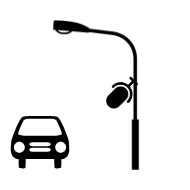
\includegraphics[width=4cm]{../Images/setup_side_view.drawio.png} }}%
    \qquad
    \subfloat[\centering Top down view]{{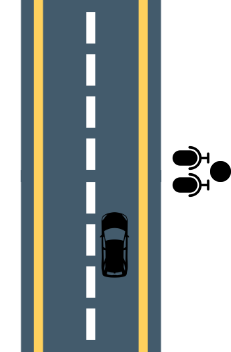
\includegraphics[width=4cm]{../Images/setup_top_down_view.drawio.png} }}%
    \caption{Baseline's microphone setup}
    \label{fig:baseline_setup}
\end{figure}

We also need to record a video of the vehicle to have a ground truth to annotate the dataset. Vehicle recordings are the most crucial part of the baseline. We need to design a system that will allow us to record vehicles from the street and save the data. We designed the system managing the data recording and storage with two microphones, a camera, an embedded system, and a server to store the recordings. This system is shown in Figure \ref{fig:recording_system_design.drawio}.

\begin{figure}[H]
    \centering
    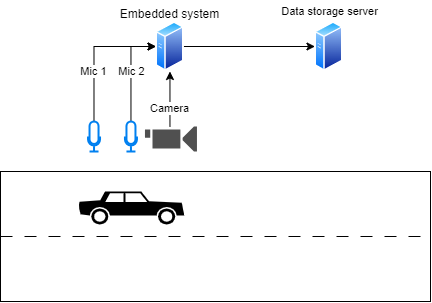
\includegraphics[width=.8\textwidth]{../Images/recording_system_design.drawio.png}
    \caption{Recording system design}
    \label{fig:recording_system_design.drawio}
\end{figure}

We defined two seconds of recording as our sample length. We chose this length arbitrarily, mainly because it is long enough to have a vehicle passing by the microphones and short enough to have a reasonable size for the dataset.

Overall, the baseline provides a context to develop further a concept of an accurate sound source localization system for outdoor space.

\subsection{Dataset conception}
\label{sec:dataset_conception}

The dataset is the most crucial part of the baseline. We can determine the dataset's characteristics based on the analysis of the section \ref{sec:datasetsSSL}. The dataset needs to contain the sound recorded by the microphone and the position of the sound source. To simplify the problem, we will use four classes as the main classification challenge in the project. The classes are the following:

\begin{itemize}
    \item  \textit{left\_to\_right}: The vehicle goes from the left to the right of the microphone.
    \item  \textit{right\_to\_left}:  The vehicle goes from the right to the left of the microphone.
    \item  \textit{no\_cars}:  No vehicles pass by the microphone.
    \item  \textit{multiple\_cars}:  Multiple vehicles pass by the microphone.
\end{itemize}

By adding a camera to the system in section \ref{sec:vehicle_recordings}, we can use the image captured by the camera to determine the ground truth of the sound source's position. The camera's position is the same as the microphone's position, and the camera is facing the road. These classes allow the creation of a dataset without precisely recording the vehicle's position. The \textit{no\_cars} and \textit{multiple\_cars} are here to ensure we will have a complete dataset, as with these four classes, we can cover every possible scenario recorded by the microphones and don't need to cherry-pick only the recordings that match our classification system. 

We also used only two classes at the beginning of the project to ensure the concept's functionality when installing the system. These classes are the following:

\begin{itemize}
    \item  \textit{left\_to\_right}:  The vehicle goes from the left to the right of the microphone.
    \item  \textit{right\_to\_left}:  The vehicle goes from the right to the left of the microphone.
\end{itemize}

\subsubsection{Recorded data design}

The input data needs to be an audio signal. Based on the analysis in section \ref{subsec:audio_file_format}, we use the Waveform Audio File Format with pulse-code modulation to represent our audio signal. With this representation, we obtain a vector of floating point numbers representing the audio signal. Since we record multiple channels simultaneously, we can consider the channels as another vector dimension. We can then represent the audio signal as a matrix of floating point numbers.

\section{Convolutional Neural Network design for Sound Source Localization}
\label{sec:cnn_design_for_ssl}

For our baseline, we use a convolutional neural network to predict the position of the sound source. We use a convolutional neural network because, based on the analysis in section \ref{sec:cnn_for_ssl}, it is the most common neural network architecture for image classification and hence for sound source localization. We can use the spectrograms as image input and the convolutional neural network to classify the spectrograms.

The network design is composed of a feature extraction part and a classifier part. The feature extraction part comprises convolutional layers, ReLU, and pooling layers. The classifier part is composed of fully connected layers. We use the feature extraction part to extract the features from the spectrograms and the classifier part to classify the features extracted. The full architecture is shown in Figure \ref{fig:baseline_feature_extraction}.

\begin{figure}[H]
    \centering
    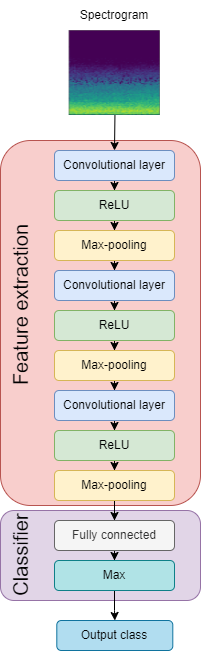
\includegraphics[width=.25\textwidth]{../Images/cnn_architecture_design.drawio.png}
    \caption{Baseline feature extraction}
    \label{fig:baseline_feature_extraction}
\end{figure}

The feature extraction part comprises three blocks of one convolution, one ReLU, and one Max-pooling. The convolutional layers extract the features from the spectrograms. The ReLU layers introduce non-linearity in the network. The pooling layers reduce the dimensionality of the network. The classifier part is composed of one fully connected layer. The fully connected layer classifies the features extracted by the feature extraction part. 

\section{Simulation concept design}
\label{sec:simulation_concept_design}

Since there are two main datasets in the project, we call the dataset described in section \ref{sec:dataset_conception} real-life dataset and the one described in this section simulation dataset. 

To improve the classification score of the baseline, we need to have more data. Multiple possibilities are available to achieve this goal. We can record more data, but it is time-consuming and expensive. We can also use a simulation to generate new data. In this project, we use a simulation to generate new recordings to add to the training dataset to achieve a better classification score on the baseline. The simulation comprises the same elements in the recording system in section \ref{sec:vehicle_recordings} except we simulate them. The simulation design is shown in Figure \ref{fig:simulation_system_design.drawio}.

\begin{figure}[H]
    \centering
    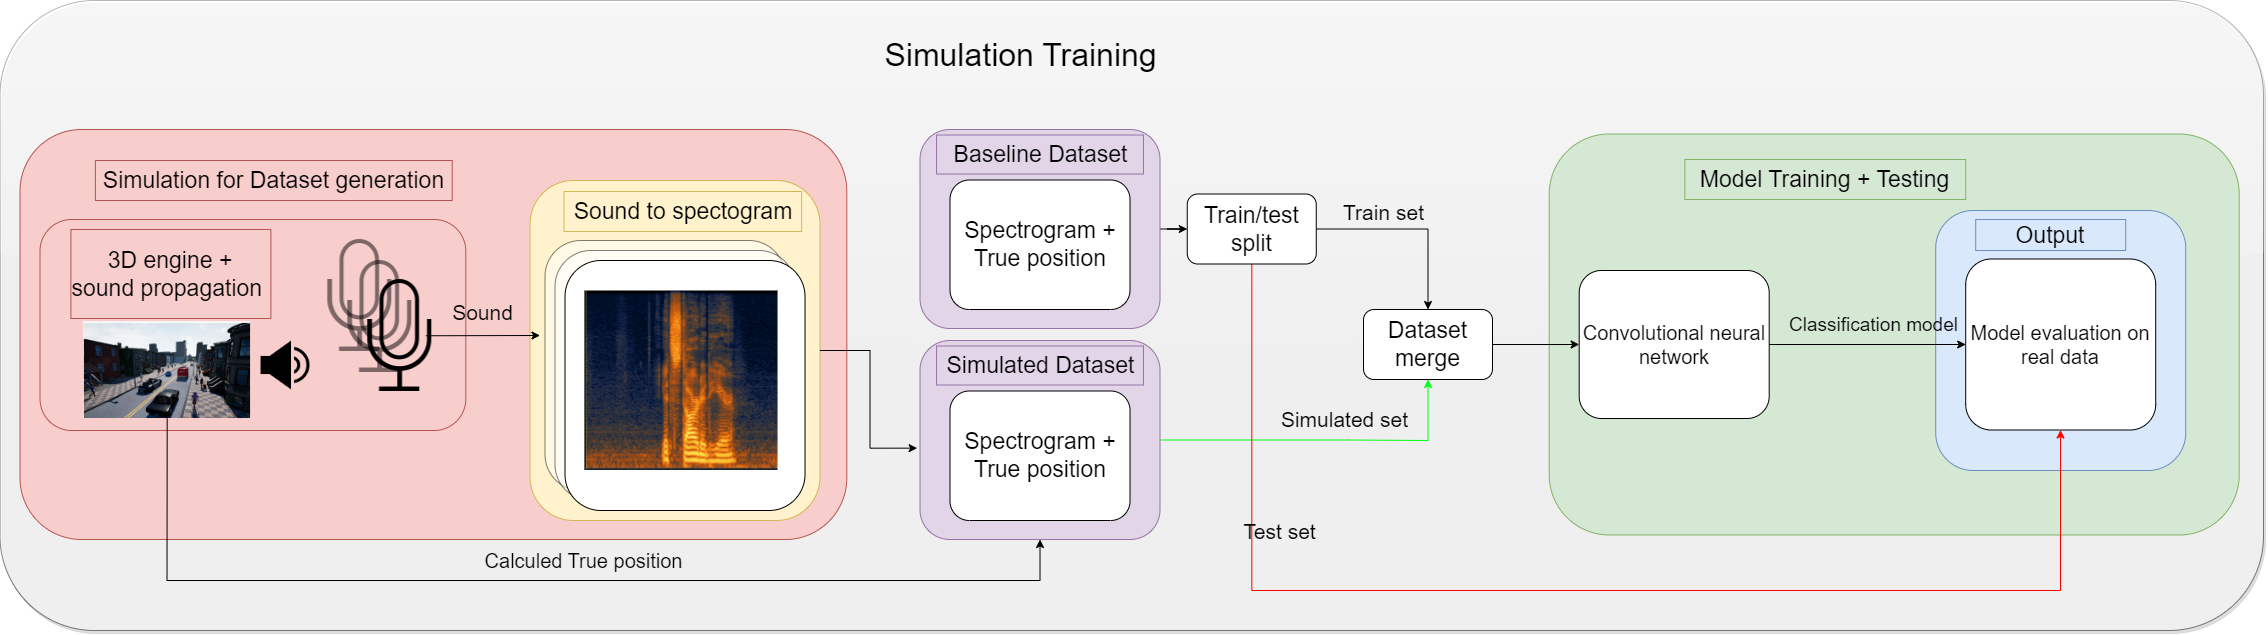
\includegraphics[width=1\textwidth]{../Images/simulation_training_design.drawio.png}
    \caption{Simulation system design for training}
    \label{fig:simulation_system_design.drawio}
\end{figure}

There are differences with the baseline system. The main one is that we generate the data in a simulation. The second is that there is no need to annotate the dataset since we know the position of the sound source in the simulation, and we can deduce the position of the sound directly from the simulation. The last one is that we add the dataset generated by the simulation to the trainset of the baseline but not to the test set. This process allows us to understand better the simulation's impact on the real-life dataset classification score.

The main advantages of the simulation are that we can generate as much data as we want. We can generate data for any position of the sound source. The simulation is composed of a vehicle, a microphone, and a camera. Based on the section \ref{sec:dataset_conception}, we want to generate data for the classes \textit{left\_to\_right} and \textit{right\_to\_left}. We can generate data for the class \textit{left\_to\_right} by placing the vehicle on the microphone's left and moving it to the right. We can generate data for the class \textit{right\_to\_left} by placing the vehicle on the right of the microphone and moving it to the left. We did not generate data for the classes \textit{no\_cars} and \textit{multiple\_cars}.

\subsection{Generalization aspect of the simulation}

Simulation is a tool to generate data. But we must be cautious because the simulation can generate data that does not represent real-life data. If the simulation generates data that does not represent real-life data, the classification score on the real-life data will be low.

For the simulation to best generalize and better represent real-life data, we need to add randomness to the simulation in multiple ways. 

\paragraph{Random speed}

The vehicle's speed is not constant in real life, and we need to add randomness to the vehicle's speed in the simulation. We can add randomness to the vehicle's speed by varying the speed assigned at the beginning of the simulation. 

\paragraph{Random path}

At the beginning of the simulation, we define multiple points as possible start and end points for the vehicle journey. The vehicle's path is generated by randomly choosing a start and end point. We can then generate the vehicle's path by drawing a straight from the start to the end. This method matches the real-life scenario where the straight road in front of the HEIA-FR building constrains the vehicle's path. 

\paragraph{Random starting time}

The vehicle's arrival time is not constant in real life. We add randomness to the vehicle's starting time in the simulation to match the real-life cases. We achieve it by varying the vehicle's waiting time at the simulation's beginning.

\paragraph{Random engine noise}

We need to assign an engine sound to the vehicle during the simulation to record the vehicle with the microphone. There are many vehicles in real life and many different engine noises. We reproduce this by randomly choosing an engine noise at the beginning of the simulation and playing it during the simulation. 

\paragraph{Random background noise}

We add randomness to the background noise by randomly choosing a noise track at the beginning of the simulation and playing it during the simulation.

\subsection{Simulation software design}

The simulation generates audio data by playing scenarios and recording the sound generated. In the simulation, we represent the comportment analyzed in section \ref{sec:baseline_analysis}.

\section{Adversarial Attack design}
\label{sec:adversarial_attack_design}

Based on the analysis in section \ref{sec:adversarial_attacks}, we can use an adversarial attack to fool the model designed in section \ref{sec:cnn_design_for_ssl}. This project uses the Fast Gradient Sign Method (FGSM) to generate adversarial inputs. The FGSM is a white-box attack meaning that we need the model's parameters to generate the adversarial inputs. Once we finish training the model, we can calculate the loss function's gradient concerning the input to find the direction that maximizes the loss function. Once we find the direction, we can add a perturbation multiplied by a value of epsilon to the input to generate the adversarial input. 
Once we generate adversarial inputs, we test them on the model to see how it reacts. We realize the attack on a specific value of epsilon. We can try to attack the model with different epsilon values to see how much noise is needed for the model to fail. We analyzed the results by comparing them with the baseline model's results.

\subsection{Audio reconstruction design}

Realizing the adversarial attack by modifying the spectrogram input is not enough to have a negative impact if we use the model for inference in a real-life scenario. Since the system designed in section \ref{sec:baseline_design} uses microphones as input, we need to transform the adversarial spectrogram back to audio. We can then play the audio on a speaker in front of the baseline system to see if the model still fails after the reconstruction of the audio signal.

\subsection{Adversarial attack protection design}

Once we generate the adversarial audio signal, we must again play it through a speaker and the microphone. We can analyze the adversarial audio signal before the classification and try detecting an attempted attack. We can use a classic CNN to classify the type of sound recorded. We can then use the classification score to detect an attempted attack.
\newpage{\pagestyle{empty} \cleardoublepage}


\chapter{Realization}
\label{ch:setup}

\section{Simulation model creation}

\subsection{Microsoft Project plugin}

\subsection{Unity plugin}

\section{Dataset creation}

\subsection{Microphone installation}

\subsection{Embedded system setup and access}

\subsection{Data transmission}

\subsection{Data recording and storage}

\section{Neural Network for Sound Source Localization}

\subsection{Dataset preparation}

\subsection{Neural Network architecture}

\subsection{Training}

\section{Adversarial Attack}

\subsection{Fast Gradient Signed Method implementation}


\newpage{\pagestyle{empty} \cleardoublepage}


\chapter{Results}
\label{ch:results}
\newpage{\pagestyle{empty} \cleardoublepage}


\chapter{Conclusions and Future Work}
\label{ch:conclusions}

\section{Objectives fullfillment}

Based on the chapter \ref{ch:results}, objectives 1, 2, 3, and 5 are fulfilled. Objective 4 is partially fulfilled. 

\section{Future Work}

We created the project for the master's thesis. We were not sure where it would lead us. After the results obtention, we can assume that we set the baseline, and other projects can use it to improve the results. A bachelor's thesis has already begun based on the baseline defined in this project. 

\subsection{Adding more microphones to the recording system}


Two microphones might not be enough for a machine learning algorithm to differentiate a sound from the left or the right. The next could be to improve the recording system by adding more microphones. This improvement would modify the dataset by adding dimensions. The current system is limited to two microphones. The system should be able to record four or more microphones. By adding channels to the audio signal, we augment the input dimension of the convolutional neural network, and we can better train it, thus improving the results.

\subsection{Labelization of more data}

Currently, the dataset only comprises a bit more than 2000 samples. By labeling more data, we can compare the results and see if the results are improving. If they improve, we can assume that the dataset needs to be way bigger for the machine learning algorithm to generalize the problem.

\subsection{Adding more classes}

The current baseline is only able to differentiate between four classes. The next step is to add more classes to the dataset. The classes could be more zones that the model would have to discern. Adding classes would also increase the problem's complexity and require more data to train the model. But it could provide a better tool to build a product we could use in real situations.

\subsection{Sound Propagation Simulation}

The sound propagation simulation was an important part of the project and is not performing well enough. The next part of improving the simulation is the implementation of a real sound propagation that simulates the time needed for the sound to reach the microphone directly into the engine and allows the use of multiple microphones at the same time while managing effects like Doppler occurring when the sound source is moving relatively to each microphone.

Not generating data for the \textit{no\_car} and the \textit{multiple\_cars} could have been an error. 

\subsection{Sound Propagation Simulation bachelor's thesis}

A thesis named \textit{SimSound3D} has started in the HEIA-FR. The goal of this thesis is to improve the sound propagation simulation. They will base their thesis on the work done in this project. At the moment, they have chosen to try to use the Unreal Engine to simulate sound propagation. The student claims to be able to record from multiple positions simultaneously. If the thesis succeeds, it could greatly improve the project.

\subsection{Advanced adversarial attack}

The current adversarial attack is a simple, inefficient attack in our situation. The next step is to improve the attack by using more advanced attacks. The patch attacks presented in [Generative Dynamic Patch Attack]\cite{li2021generative} could change a zone in the image, thus, making it easier to transform it back to an audio signal without adding lots of noise on the whole spectrogram. This process could improve the attack's efficiency and make it more realistic.

\subsection{Dataset publication}

Since we created a dataset containing more than 2000 labeled samples, we could publish it. Other researchers could use the dataset for their projects. The machine learning community could also use the dataset to improve the project results.

\section{Specification self-assessment}

At the beginning of the project, the specification was going more toward emergency vehicle detection. During the project, we modified the project's objectives to a more generic sound source localization and distance estimation. We adapted the specification to the new objectives. 

The planning was designed with three epic deadlines during the project to represent a cyclic workflow. Although the three epic deadlines did not represent three different project realization cycles, they were still useful for providing a global view during the project. The tasks defined in the planning were well followed.

The specification file was a good base to start the project and was a good way to have a global view of what we wanted to do.

\section{Personal conclusion}

It is a great opportunity to work on a project that tries to regroup every part of the IT domain, from embedded systems to machine learning. Even if this project was big and sometimes felt like multiple projects at once, it was a great experience to work on it. I learned much about the different domains and technologies, especially adversarial attacks. I also learned how to manage a project. I am happy with the results, and I am looking forward to seeing the next steps of the project.

\newpage{\pagestyle{empty} \cleardoublepage}


\begin{appendix}
\chapter{Appendix}
\newpage
\section{Specification}
\label{appendix:specification}
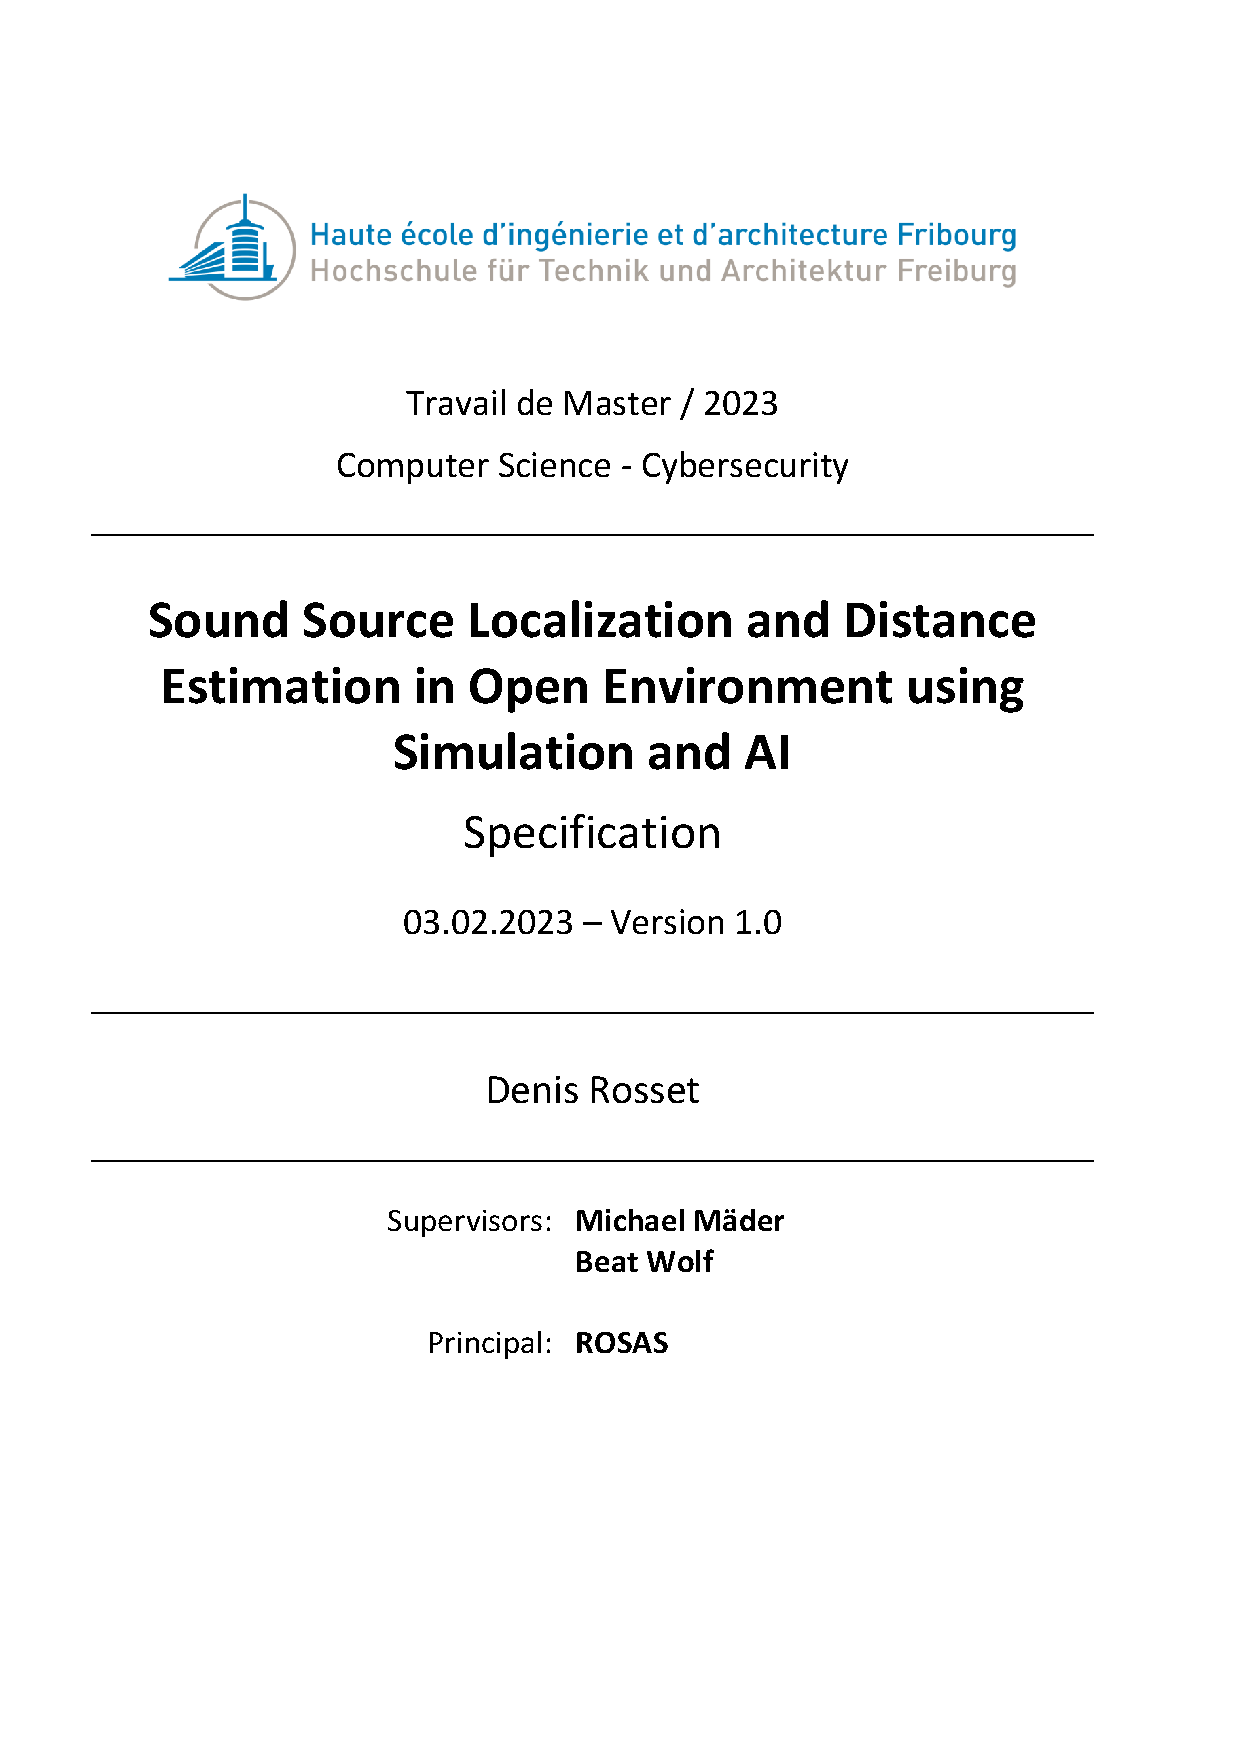
\includepdf[pages=-]{../specification/specification.pdf}

\newpage{\pagestyle{empty} \cleardoublepage}
\end{appendix}

\addcontentsline{toc}{chapter}{\numberline{}List of Tables}
\listoftables

\addcontentsline{toc}{chapter}{\numberline{}List of Figures}
\listoffigures

\addcontentsline{toc}{chapter}{\numberline{}Bibliography}

\bibliography{Bibliography/libs}
\bibliographystyle{unsrt}

%END Doc
%-------------------------------------------------------

\end{document}

